\capitulo{3}{Conceptos teóricos}
\section{Encriptado de contraseñas}
Se detectó un fallo de seguridad grave y es que las contraseñas no se cifraban para los nuevos usuarios por lo tanto para solventar ese problema se implementó un sistema de encriptado de contraseñas.\\
Para ello me informé de los posibles cifrados.
\subsection{password\_hash}
Esta función de PHP crea un hash de contraseña usando un algoritmo de hash fuerte de único sentido.\\
Para entender esta función me hizo falta aprender lo que es un hash.\\
Una función criptográfica hash es un algoritmo matemático que transforma cualquier bloque arbitrario de datos en una nueva serie de caracteres con una longitud fija. Independientemente de la longitud de los datos de entrada, el valor hash de salida tendrá siempre la misma longitud.\cite{definicionHash}
Password\_hash() se emplea para crear un hash con una cadena dada como primer argumento utilizando el algoritmo pasado como segundo argumento. 
Se puede elegir entre estos dos algoritmos para el encriptado:
\begin{description}
    \item [PASSWORD\_DEFAULT] Usa el algoritmo bcrypt. Esta constante está diseñada para cambiar siempre que se añada un algoritmo nuevo y más fuerte a PHP. Por esto la longitud de la encriptación puede variar según cambia el algoritmo.
    \item [PASSWORD\_BCRYPT] Usa el algoritmo CRYPT\_BLOWFISH para crear el hash. Produce un hash usando el identificador "\$2y\$". El resultado siempre será un string de 60 caracteres, o FALSE en caso de error.
\end{description}
Para comprobar que una contraseña introducida en el login coincide con el hash guardado en la base de datos se usa la función password\_verify().\cite{passwordHash}
\imagen{imagenes/Ejpasshash}{Ejemplo de la utilización de password\_hash()}
\subsection{crypt}
Esta función tiene un funcionamiento muy similar que password\_hash().\\
Se le pasan dos parámetros, el string que queremos encriptar y un string de salt para la base del hash.\cite{crypt} A continuación se define lo que es un string salt.\\
En criptografía, la sal o salt en inglés comprende bits aleatorios que se usan como argumento en una función que crea contraseñas. El otro argumento es el string que queremos codificar. El string salt también puede usarse como parte de una clave en un cifrado u otro algoritmo criptográfico. A veces se usa como salt el vector de inicialización, un valor generado previamente.
Las claves con sal complican los ataques de diccionario que cifran cada una de las entradas del mismo: cada bit de sal duplica la cantidad de almacenamiento y computación requeridas.\cite{salt}
\subsection{Hash de Laravel}
Laravel tiene una clase Hash que permite el encriptado de contraseñas usando los algoritmos Bcrypt y Argon2.\\
Bcrypt es una excelente opción para hacer hash de contraseñas porque su factor de trabajo es ajustable, lo que significa que el tiempo que lleva generar un hash puede incrementarse a medida que aumenta la potencia del hardware. Cuando se procesan contraseñas, la lentitud es buena. Cuanto más tiempo tarda un algoritmo en codificar una contraseña, más tardan los usuarios malintencionados en generar todas las cadenas posibles que pueden utilizarse en ataques de fuerza bruta contra aplicaciones.\cite{HashLaravel}
\imagen{imagenes/HashLaravel}{Encriptación de contraseñas en mi aplicación}
Después de informarme de todas las posibilidades que había para el cifrado, elegí la clase hash de Laravel usando el algoritmo bcrypt.\\
Escogí esta porque me pareció la más actual y documentada y, además pertenece a Laravel por lo que pensé que sería mas adecuada para mi trabajo. En cuanto al algoritmo bcrypt me pareció bastante fiable y eficaz al utilizarse en otros sistema de elevada relevancia como OpenBSD y algunas distribuciones de Linux.
 \section{Estructura de los datos del INE}
El Instituto Nacional de Estadística proporciona un servicio que permite descargar los datos que nos ofrece en formato JSON. Para ello debemos crear una petición en forma de url para después guardar esos datos e introducirlos en nuestra base de datos.\\
La información de esta plataforma proviene de dos fuentes: la base de datos de difusión Tempus3 y el repositorio de ficheros PC-Axis.\\
 \subsection{Creación de la url}
 Para comprender este paso hace falta saber cómo es la estructura de una petición url para el servicio de datos abiertos del INE. \cite{ine:urljson}\\
 \imagen{imagenes/urlJSON}{Estructura de la url}
Los campos que aparecen entre llaves, \{ \}, son obligatorios.\\
Los campos que aparecen entre corchetes, [ ], son opcionales y cambian en relación a la función considerada.\\
Descripción de cada uno de ellos
\begin{description}
	\item [idioma] ES para español e EN para inglés. Por defecto está puesto el español.\\
	\item [función] Funciones implementadas en el sistema para poder realizar diferentes tipos de consulta en función del tipo de fuente, Tempus3 o PC-Axis, y del elemento que se quiere obtener. Hablaré de estas funciones más adelante en la sección de "Metadatos y datos".\\
    Funciones para la obtención de datos de Tempus3:
         \begin{description}
         \item [Operaciones] OPERACIONES\_DISPONIBLES, OPERACIÓN.
         \item [Variables] VARIABLES, VARIABLES\_OPERACION.
         \item [Valores] VALORES\_VARIABLES, VALORES\_VARIABLEOPERACION.
         \item [Tablas] TABLAS\_OPERACION, GRUPOS\_TABLA.
         \item [Series] SERIE, SERIES\_OPERACION.
         \item [Publicaciones] PUBLICACIONES, PUBLICACIONES\_OPERACION.
         \item [Datos] DATOS\_SERIE, DATOS\_TABLA.
         \end{description}
    Función para la obtención de datos del repositorio de ficheros PC-Axis:\\ Al ser éste un formato para difundir tablas estadísticas, la única función implementada es la siguiente:
         \begin{description}
         \item [Datos] DATOS\_TABLA
         \end{description}
    \item [inputs] Identificadores de los elementos de entrada de las funciones. Estos inputs varían en base a la función utilizada.
    Existen dos tipos de repositorios de los que el INE saca sus datos; los repositorios de tablas Tempus3 y los de PC-Axis.
    \imagen{imagenes/idTempus3}{Identificador de las tablas Tempus3}
    \imagen{imagenes/idPcAxis}{Identificador de las tablas PC-Axis}
    \item [parámetros] Los parámetros en la URL se establecen a partir del símbolo ?.\\
    Cuando haya más de un parámetro, el símbolo \& se utiliza como separador.\\
    No todas las funciones admiten todos los parámetros posibles. Por ello haremos una clasificación para explicarlos mejor:  
     \begin{enumerate}
        \item Parámetros comunes a todas las funciones
            \begin{description}
            \item [page] Si hay más de 500 elementos, la consulta se divide en páginas. Esta opción nos permite seleccionar la página que queremos visualizar.
            \item [download] Para descargarnos el fichero JSON.
            \item [det] Este parámetro da más detalles de la información mostrada.
            \item [tip] Cambia la forma de mostrar la información.
            \end{description}
        \item Parámetros para la petición de datos
            \begin{description}
                \item [date] Filtra los datos por fecha; fecha concreta, lista o rango de fechas.
                \item [nult] Devuelve los últimos n datos. Ejemplo: nult=4 devuelve los 4 últimos datos.
            \end{description}
        \item Parámetros para la obtención de datos y metadatos en base al ámbito geográfico
            \begin{description}
                \item [geo] Con geo = 1 para provincias, municipios u otras desagregaciones y geo = 0 para datos nacionales.
            \end{description}
        \end{enumerate}
\end{description}
 Para facilitar el trabajo a los usuarios de la aplicación, la petición url se genera automáticamente a partir de la url de la página del INE donde se encuentren los datos que queremos.
 \imagen{imagenes/Ine}{Ejemplo de una tabla del INE}
 \imagen{imagenes/urlINE}{Ejemplo de la url del INE}
 El usuario copia y pega esta dirección y la aplicación la traduce a una petición url de los datos en forma de JSON automáticamente.
\subsection{Metadatos y datos}
Los datos y los metadatos hacen referencia al apartado {función} de la petición url antes vista.
\subsubsection{Metadatos}
La petición de metadatos sólo está disponible para el sistema Tempus3. Se pueden consultar estos tipos de metadatos:
\begin{enumerate}
    \item Operaciones\\ Para consultar todas las operaciones disponibles:\\ OPERACIONES\_DISPONIBLES.\\ La petición url sería esta:\\ https://servicios.ine.es/wstempus/js/ES/OPERACIONES\_DISPONIBLES\\ Y el output sería un JSON con información sobre todas las operaciones estadísticas disponibles como por ejemplo la del índice de precios de consumo\\
    \{"Id":25, "Cod\_IOE":"30138", "Nombre":"Índice de Precios de Consumo (IPC)", "Codigo":"IPC"\}.\\
    Para consultar una operación en concreto se usa la función OPERACIÓN y como input para identificar la operación se utilizan los códigos que sacamos del output anterior. Por ejemplo para consultar la operación del índice de precios de consumo (IPC), se pueden usar tres input diferentes:  IOE30138, IPC o 25.
    \item Variables\\
    Para obtener todas las variables: VARIABLES\\ https://servicios.ine.es/wstempus/js/ES/VARIABLES\\
    Para obtener las variables de una operación concreta se utiliza como función VARIABLES\_OPERACIÓN y como input cualquiera de los códigos de identificación de la operación antes mencionados. Ejemplo: https://servicios.ine.es/wstempus/js/ES/VARIABLES\_OPERACION/IPC \\
    \item Valores\\
    Se puede acceder a los valores de una variable con la función VALORES\_VARIABLE y con el input correspondiente al código de la operación.\\
    También se muestran los valores que tiene una variable para una operación en concreto con la función VALORES\_VARIABLEOPERACIÓN y el input de la operación que queramos mostrar. 
    \item Tablas\\
    Para obtener todas las tablas asociadas a una operación usamos TABLAS\_OPERACIÓN con el código identificativo de la operación como input.\\
    También podemos mostrar los grupos de una tabla con GRUPOS\_TABLA y usar VALORES\_GRUPOSTABLA para obtener los valores de cada uno de los grupos de una tabla usando además su código identificativo como output. Ejemplo:\\
    https://servicios.ine.es/wstempus/js/ES/GRUPOS\_TABLA/22350\\
    Con esta petición url sacamos los grupos de la tabla con el identificador 22350.\\
    Una fila del output correspondiente a los índices por comunidades autónomas sería esta:\\
    \{"Id":22350, "Nombre":"Índices por comunidades autónomas: general y de grupos ECOICOP", "Codigo":"2016\_NAC-CCAA", "FK\_Periodicidad":1, "FK\_Publicacion":8, "FK\_Periodo\_ini":1, "Anyo\_Periodo\_ini":"2002", "FechaRef\_fin":"null", "Ultima\_Modificacion":1607673600000\}\\
    Y para extraer los valores de ese grupo utilizaríamos la petición:\\
    \small servicios.ine.es/wstempus/js/ES/VALORES\_GRUPOSTABLA/22350/81497\\
    \item Series\\
    Una serie es un conjunto de observaciones medidas en un instante de tiempo determinado.\\ 
    La API JSON del INE nos permite usar las siguientes funciones para sacar información sobre las series:  
    \begin{description}
            \item [SERIE]
            Para formar esta url se usa la función y el input identificativo de la serie. Como output sale la información de la serie requerida.\\
            \item [SERIES\_OPERACION]
            La url se construye de la misma manera pero el output de esta son las series pertenecientes a una determinada operación.\\
            \item [VALORES\_SERIE]
            Con esta función obtenemos información de los metadatos que definen a la serie.\\
            \item [SERIES\_TABLA]
            Utilizando esta función conseguimos datos sobre las series de una tabla de la que pasamos el código identificativo como input.\\
            \item [SERIE\_METADATAOPERACION]
            Esta opción sirve para obtener información detallada sobre un conjunto de datos preciso de una operación. La operación se pasa como un input mediante su identificador.\\
    \end{description}
    \item Publicaciones\\
    Para este tipo de metadatos hay tres funciones muy sencillas: PUBLICACIONES que muestra una lista de todas las publicaciones existentes, PUBLICACIONES\_OPERACION que muestra las publicaciones de una determinada operación que se pasa como input y PUBLICACIONFECHA\_PUBLICACION que saca las fechas en las que se han añadido nuevos datos a una determinada publicación.\\
\end{enumerate}
\subsubsection{Datos}
Es la parte que realmente se trata dentro de la aplicación. Existen varios tipos:\\
\begin{enumerate}
    \item DATOS\_SERIE\\
    Con esta función obtenemos datos de una serie en concreto.\\
    \item DATOS\_TABLA\\
     Información y datos de las series contenidas en la tabla. Los valores vienen clasificados en función del periodo y del año. Puesto que en esta aplicación la forma de clasificar los datos es en tablas, esta función será la que usaremos.\\ 
     \item DATOS\_METADATAOPERACION\\
      Esta opción sirve para obtener información sobre un conjunto de datos preciso de una operación. La operación se pasa como un input mediante su identificador.\\
\end{enumerate}
\section{Algoritmos de predicción de datos}
Para la estimación de datos a futuro se ha utilizado la librería Rubix ML desde la que se pueden usar múltiples algoritmos para la predicción de los datos. Se distinguen dos grandes grupos: Clasificadores y regresores. A continuación explicaré ambos.
\subsection{Clasificadores}
Estos algoritmos predicen datos categóricos basados en la información con la que han sido entrenados. No entraré en más detalle ya que no se usan en el proyecto.
\subsection{Regresores}
Los estimadores de tipo regresor se usan para predecir datos continuos. Son los siguientes:
\begin{description}
    \item [Adaline] Es un tipo de red neuronal artificial caracterizada por tener múltiples nodos los cuales aceptan muchos inputs para generar un solo output \cite{Adaline}. Las variables que utiliza son:
    \begin{description}
        \item [x] Es el vector que contiene los datos de entrada.
        \item [w] Vector que indica la fuerza de conexión entre los valores de entrada y la neurona.
        \item [n] Número de inputs.
        \item [\begin{math}\theta \end{math}.] La constante.
        \item [y] Datos de salida.
    \end{description}
    \begin{figure}[!h]
		\centering
		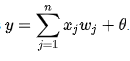
\includegraphics[width=0.3\textwidth]{imagenes/adaline}
		\caption{Ecuación}\label{fig:Ecuación}
	\end{figure}
	\item [Regression Tree] Consiste en un árbol de decisión que se va bifurcando según los posibles resultados de una serie de decisiones relacionadas. Los parámetros son los siguientes:
	\begin{description}
	    \item [maxHeight] Altura máxima del árbol.
	    \item [maxLeafSize] Máximo número de decisiones que una hoja puede tener.
	    \item [maxFeatures] Máximo número de columnas a considerar al elegir una decisión.
	    \item [minPurityIncrease] Aumento mínimo de pureza necesario para que un nodo no se pode durante el crecimiento del árbol.
	\end{description}
	\item [Extra Tree Regressor] Es igual que el anterior pero se diferencian en que este modelo escoge la siguiente decisión de forma aleatoria en vez de buscar el mejor valor en una serie de datos. Son muy rápidos de construir pero sus resultados son muy variables. Los parámetros son los mismos.
	\item [KNN] K Nearest Neighbors (KNN) es un algoritmo de fuerza bruta que localiza el k más cercano de los valores de entrada con los que se ha entrenado para hacer su predicción. Tiene tres parámetros:
	\begin{description}
	    \item[k] El número de vecinos a considerar al hacer la predicción.
	    \item[weighted] Booleano que indica si se debe considerar la distancia de los vecinos más cercanos al hacer la predicción.
	    \item[kernel] El kernel que se va a usar para computar la distancia entre los puntos de referencia.
	\end{description}
	\item[K-d Neighbors Regressor] Es una implementación rápida del algoritmo anterior. Usa un árbol binario con reconocimiento espacial para la búsqueda de vecinos más cercanos. Kd Neighbors Regressor funciona localizando la vecindad de una muestra mediante una búsqueda binaria y luego realiza una búsqueda de fuerza bruta solo en las muestras cercanas o dentro de la vecindad de la muestra desconocida.  La principal ventaja de Kd Neighbors sobre la fuerza bruta KNN es la velocidad de inferencia. Parámetros:
	\begin{description}
	    \item[k] El número de vecinos a considerar al hacer la predicción.
	    \item[weighted] Booleano que indica si se debe considerar la distancia de los vecinos más cercanos al hacer la predicción.
	    \item[tree] Árbol usado para ejecutar las búsquedas de los vecinos cercanos.
	\end{description}
	\item [MLP Regressor] Es una red neuronal multicapa con un output continuo adecuado para problemas de regresión.  El regresor de perceptrón multicapa (MLP) es capaz de manejar problemas complejos de regresión no lineal formando representaciones de orden superior de las características de entrada utilizando capas ocultas intermedias definidas por el usuario.\\
	El MLP también tiene instantáneas de red y monitoreo del progreso.
\end{description}
\section{Integración continua}
La integración continua es una práctica de ingeniería de software que consiste en hacer integraciones automáticas de un proyecto lo más a menudo posible para así poder detectar fallos cuanto antes. Entendemos por integración la compilación y ejecución de pruebas de todo un proyecto.\cite{IntegracionContinua}
Ventajas de usar la integración continua 
\begin{itemize}
    \item Capacidad de detección de problemas temprana, lo que facilita su solución.
    \item Disponibilidad en cualquier momento de distintas versiones.
    \item Ejecución inmediata de las pruebas unitarias.
    \item Monitorización continua de las métricas de calidad del código del proyecto.
\end{itemize}
Para usar la integración continua en mi proyecto he usado la herramienta codacy que analiza el código y realiza un informe cada vez que ocurre algún cambio en este y los test de Laravel dusk que se ejecutan para ver que todo sigue funcionando correctamente.\\


 